\section{Триггеры}

\subsection*{Постановка задачи}
На основе представления \textbf{car\_stats} создаётся таблица с теми же
показателями. Триггеры должны поддерживать согласованность её данных при
изменении таблиц \textbf{car}, \textbf{alert\_event} и
\textbf{parking\_session}.

\subsection{Создание таблицы статистики}
Сначала представление переименовывается в \textbf{car\_stats\_view}, после
чего создаётся таблица \textbf{car\_stats} и заполняется данными из
представления. Порядок операций важен: представление и таблица не могут
иметь одинаковое имя.

\begin{lstlisting}[style=sqlstyle, caption={Создание и начальное заполнение таблицы статистики}, label={lst:create-car-stats}]
ALTER VIEW car_stats RENAME TO car_stats_view;

CREATE TABLE car_stats (
    car_id        INT PRIMARY KEY REFERENCES car(car_id) ON DELETE CASCADE,
    reg_number    VARCHAR(9) NOT NULL,
    alert_count   BIGINT NOT NULL DEFAULT 0,
    parking_count BIGINT NOT NULL DEFAULT 0
);

INSERT INTO car_stats (car_id, reg_number, alert_count, parking_count)
SELECT car_id, reg_number, alert_count, parking_count
FROM car_stats_view;
\end{lstlisting}

\subsection{Триггеры для таблицы автомобилей}
При добавлении автомобиля в таблице статистики создаётся строка с нулевыми
счётчиками. При изменении регистрационного номера обновляется его копия в
\textbf{car\_stats}. Перед удалением автомобиля удаляется соответствующая
строка статистики.

\begin{lstlisting}[style=sqlstyle, caption={Функция и триггеры для таблицы \texttt{car}}, label={lst:car-triggers}]
CREATE OR REPLACE FUNCTION car_stats_change()
RETURNS TRIGGER AS $$
BEGIN
    IF TG_OP = 'INSERT' THEN
        INSERT INTO car_stats (car_id, reg_number, alert_count, parking_count)
        VALUES (NEW.car_id, NEW.reg_number, 0, 0);
        RETURN NEW;
    ELSIF TG_OP = 'UPDATE' THEN
        UPDATE car_stats
        SET reg_number = NEW.reg_number
        WHERE car_id = NEW.car_id;
        RETURN NEW;
    ELSIF TG_OP = 'DELETE' THEN
        DELETE FROM car_stats
        WHERE car_id = OLD.car_id;
        RETURN OLD;
    END IF;
END;
$$ LANGUAGE plpgsql;

CREATE TRIGGER car_stats_after_insert
AFTER INSERT ON car
FOR EACH ROW EXECUTE FUNCTION car_stats_change();

CREATE TRIGGER car_stats_after_reg_number_update
AFTER UPDATE OF reg_number ON car
FOR EACH ROW
WHEN (OLD.reg_number IS DISTINCT FROM NEW.reg_number)
EXECUTE FUNCTION car_stats_change();

CREATE TRIGGER car_stats_before_delete
BEFORE DELETE ON car
FOR EACH ROW EXECUTE FUNCTION car_stats_change();
\end{lstlisting}

\subsection{Триггеры для тревожных событий}
При добавлении тревожного события счётчик \textbf{alert\_count} автомобиля
увеличивается на единицу, а при удалении --- уменьшается.

\begin{lstlisting}[style=sqlstyle, caption={Функция и триггеры для таблицы \texttt{alert\_event}}, label={lst:alert-triggers}]
CREATE OR REPLACE FUNCTION alert_event_stats_change()
RETURNS TRIGGER AS $$
BEGIN
    IF TG_OP = 'INSERT' THEN
        UPDATE car_stats
        SET alert_count = alert_count + 1
        WHERE car_id = NEW.car_id;
        RETURN NEW;
    ELSIF TG_OP = 'DELETE' THEN
        UPDATE car_stats
        SET alert_count = GREATEST(alert_count - 1, 0)
        WHERE car_id = OLD.car_id;
        RETURN OLD;
    END IF;
END;
$$ LANGUAGE plpgsql;

CREATE TRIGGER alert_event_after_insert
AFTER INSERT ON alert_event
FOR EACH ROW EXECUTE FUNCTION alert_event_stats_change();

CREATE TRIGGER alert_event_after_delete
AFTER DELETE ON alert_event
FOR EACH ROW EXECUTE FUNCTION alert_event_stats_change();
\end{lstlisting}

\subsection{Триггер для парковочных сессий}
Счётчик \textbf{parking\_count} хранит число различных зон, поэтому при
удалении одной сессии уменьшать его можно только тогда, когда у автомобиля
больше не осталось сессий в этой же зоне. Функция на
листинге~\ref{lst:parking-session-trigger} проверяет это условие до удаления
строки.

\begin{lstlisting}[style=sqlstyle, caption={Триггер удаления парковочной сессии}, label={lst:parking-session-trigger}]
CREATE OR REPLACE FUNCTION parking_session_stats_delete()
RETURNS TRIGGER AS $$
BEGIN
    IF NOT EXISTS (
        SELECT 1
        FROM parking_session
        WHERE car_id = OLD.car_id
          AND parking_zone_id = OLD.parking_zone_id
          AND parking_session_id <> OLD.parking_session_id
    ) THEN
        UPDATE car_stats
        SET parking_count = GREATEST(parking_count - 1, 0)
        WHERE car_id = OLD.car_id;
    END IF;
    RETURN OLD;
END;
$$ LANGUAGE plpgsql;

CREATE TRIGGER parking_session_before_delete
BEFORE DELETE ON parking_session
FOR EACH ROW
EXECUTE FUNCTION parking_session_stats_delete();
\end{lstlisting}

Отдельный триггер на удаление \textbf{parking\_zone} не требуется. Внешний
ключ \textbf{parking\_session.parking\_zone\_id} настроен с правилом
\textbf{ON DELETE CASCADE}; следовательно, удаление зоны удаляет связанные
парковочные сессии, а триггер \textbf{parking\_session\_before\_delete}
корректирует статистику. Это предотвращает двойное уменьшение счётчика для
одной зоны.

\subsection{Проверка работы триггеров}
Перед проверкой триггеров выполняем команду \texttt{BEGIN;} для начала транзакции. После проверки всех триггеров выполняется команда \texttt{ROLLBACK;} для отмены изменений. Чтобы не засорять базу данных тестовыми данными.

\subsubsection*{Проверка триггеров таблицы автомобилей}
Сначала добавляется тестовый автомобиль.

\begin{lstlisting}[style=sqlstyle, caption={Добавление тестового автомобиля}, label={lst:check-car-insert}]
INSERT INTO car (
    reg_number, brand, model, manufacture_year, vin, car_status_id
)
VALUES (
    'Т777ТТ78', 'Test', 'Trigger', 2026, 'VINTRIGGER0000000',
    (SELECT car_status_id FROM car_status LIMIT 1)
);
\end{lstlisting}

После добавления в таблице статистики должна появиться строка с нулевыми
счётчиками.

\begin{lstlisting}[style=sqlstyle, caption={Проверка статистики после добавления автомобиля}, label={lst:check-car-after-insert}]
SELECT cs.*
FROM car_stats cs
JOIN car c ON c.car_id = cs.car_id
WHERE c.vin = 'VINTRIGGER0000000';
\end{lstlisting}

\begin{figure}[H]
    \centering
    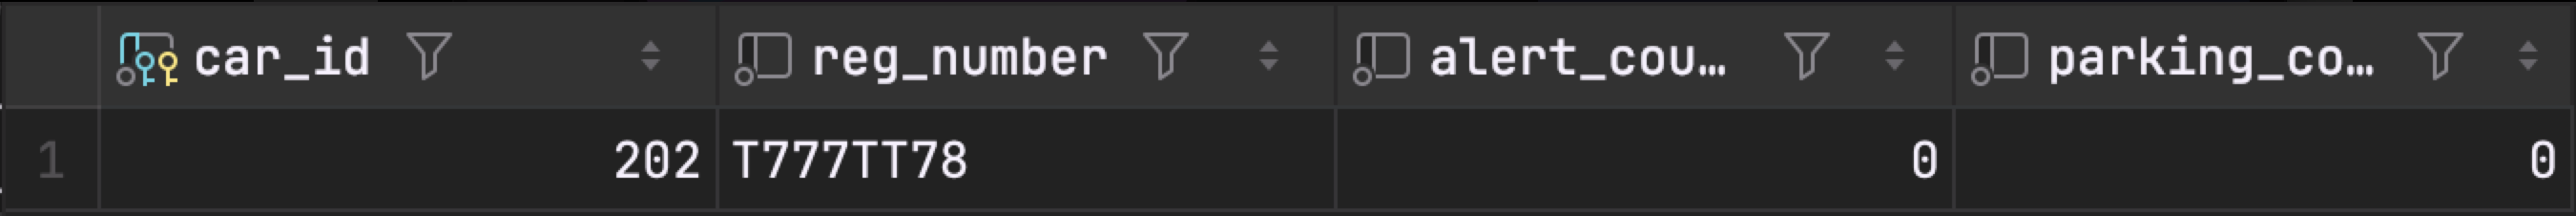
\includegraphics[width=0.6\linewidth]{myPhoto/trigger-1.png}
    \caption{Таблица \texttt{car\_stats} после добавления тестового автомобиля}
    \label{fig:trigger-1}
\end{figure}

Далее изменяется регистрационный номер автомобиля.

\begin{lstlisting}[style=sqlstyle, caption={Изменение регистрационного номера}, label={lst:check-car-update}]
UPDATE car
SET reg_number = 'Т888ТТ78'
WHERE vin = 'VINTRIGGER0000000';
\end{lstlisting}

\begin{lstlisting}[style=sqlstyle, caption={Проверка статистики после изменения номера}, label={lst:check-car-after-update}]
SELECT cs.*
FROM car_stats cs
JOIN car c ON c.car_id = cs.car_id
WHERE c.vin = 'VINTRIGGER0000000';
\end{lstlisting}

\begin{figure}[H]
    \centering
    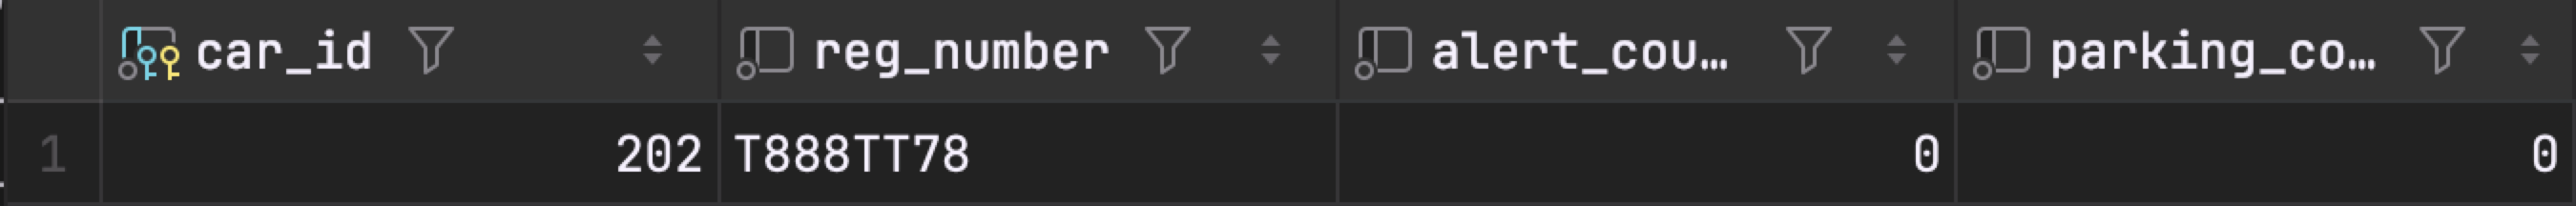
\includegraphics[width=0.5\linewidth]{myPhoto/trigger-2.png}
    \caption{Таблица \texttt{car\_stats} после изменения регистрационного номера автомобиля}
    \label{fig:trigger-2}
\end{figure}

В конце тестовый автомобиль удаляется.

\begin{lstlisting}[style=sqlstyle, caption={Удаление тестового автомобиля}, label={lst:check-car-delete}]
DELETE FROM car
WHERE vin = 'VINTRIGGER0000000';
\end{lstlisting}

\begin{lstlisting}[style=sqlstyle, caption={Проверка удаления строки статистики}, label={lst:check-car-after-delete}]
SELECT *
FROM car_stats
WHERE reg_number = 'Т888ТТ78';
\end{lstlisting}

\begin{figure}[H]
    \centering
    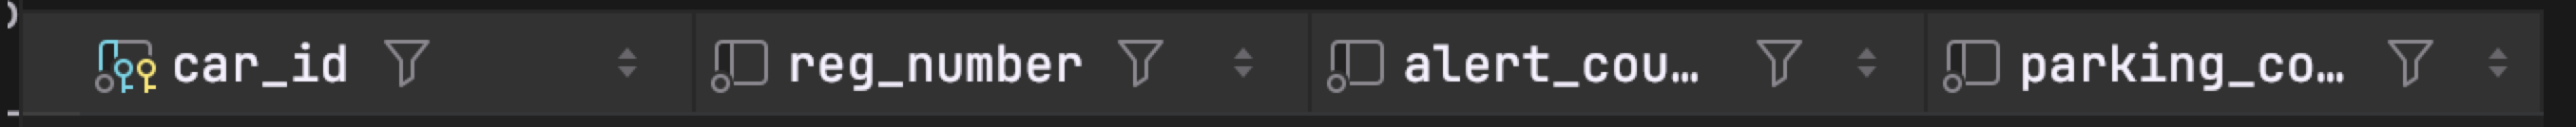
\includegraphics[width=0.5\linewidth]{myPhoto/trigger-3.png}
    \caption{Таблица \texttt{car\_stats} после удаления тестового автомобиля}
    \label{fig:trigger-3}
\end{figure}

\subsubsection*{Проверка триггеров тревожных событий}
Выберите существующий идентификатор автомобиля вместо \texttt{<car\_id>} и
сначала зафиксируйте его исходное значение \textbf{alert\_count}.

\begin{lstlisting}[style=sqlstyle, caption={Исходная статистика тревожных событий}, label={lst:check-alert-before}]
SELECT car_id, alert_count
FROM car_stats
WHERE car_id = 1;
\end{lstlisting}

\begin{figure}[H]
    \centering
    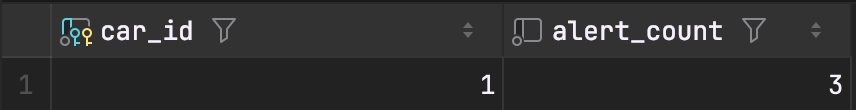
\includegraphics[width=0.5\linewidth]{myPhoto/trigger-4.png}
    \caption{Таблица \texttt{car\_stats} до добавления тревожного события}
    \label{fig:trigger-4}
\end{figure}

Для выбранного автомобиля добавляется тестовое тревожное событие. Полученный
идентификатор используется в запросе удаления.

\begin{lstlisting}[style=sqlstyle, caption={Добавление тревожного события}, label={lst:check-alert-insert}]
INSERT INTO alert_event (
    car_id, alert_event_type_id, status_id, description
)
VALUES (
    1,
    (SELECT alert_event_type_id FROM alert_event_type LIMIT 1),
    (SELECT status_id FROM alert_event_process_status LIMIT 1),
    'Тестовое тревожное событие'
)
RETURNING alert_event_id;
\end{lstlisting}

\begin{figure}[H]
    \centering
    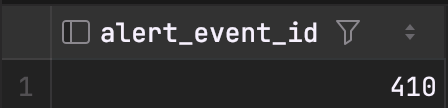
\includegraphics[width=0.5\linewidth]{myPhoto/trigger-5.png}
    \caption{Идентификатор добавленного тревожного события}
    \label{fig:trigger-5}
\end{figure}

\begin{lstlisting}[style=sqlstyle, caption={Проверка статистики после добавления события}, label={lst:check-alert-after-insert}]
SELECT car_id, alert_count
FROM car_stats
WHERE car_id = 1;
\end{lstlisting}

\begin{figure}[H]
    \centering
    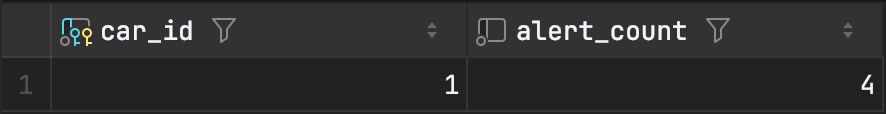
\includegraphics[width=0.5\linewidth]{myPhoto/trigger-6.png}
    \caption{Таблица \texttt{car\_stats} после добавления тревожного события}
    \label{fig:trigger-6}
\end{figure}

\begin{lstlisting}[style=sqlstyle, caption={Удаление тестового тревожного события}, label={lst:check-alert-delete}]
DELETE FROM alert_event
WHERE alert_event_id = <alert_event_id>;
\end{lstlisting}

\begin{lstlisting}[style=sqlstyle, caption={Проверка статистики после удаления события}, label={lst:check-alert-after-delete}]
SELECT car_id, alert_count
FROM car_stats
WHERE car_id = 1;
\end{lstlisting}

\begin{figure}[H]
    \centering
    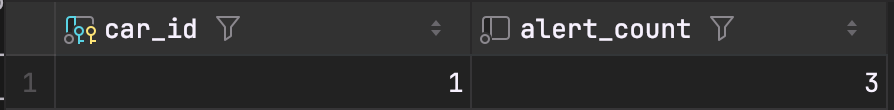
\includegraphics[width=0.5\linewidth]{myPhoto/trigger-7.png}
    \caption{Описание изображения}
    \label{fig:trigger-7}
\end{figure}

\subsubsection*{Проверка триггера парковочных сессий}
Сначала следует найти автомобиль с двумя или более сессиями в одной зоне.
Из результата нужно сохранить \texttt{car\_id} и
\texttt{parking\_zone\_id}.

\begin{lstlisting}[style=sqlstyle, caption={Поиск данных для проверки парковочных сессий}, label={lst:find-parking-session}]
SELECT
    ps.car_id,
    ps.parking_zone_id,
    COUNT(*) AS session_count
FROM parking_session ps
GROUP BY ps.car_id, ps.parking_zone_id
HAVING COUNT(*) >= 2
LIMIT 1;
\end{lstlisting}

\begin{figure}[H]
    \centering
    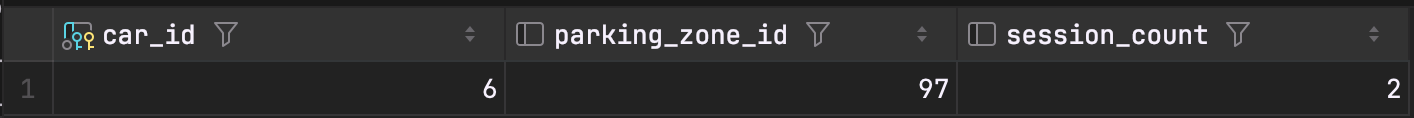
\includegraphics[width=0.5\linewidth]{myPhoto/trigger-8.png}
    \caption{Результат поиска автомобиля с двумя и более сессиями в одной зоне}
    \label{fig:trigger-8}
\end{figure}

После подстановки найденных значений отдельным запросом выводятся
идентификаторы сессий. Один из них необходимо оставить для последнего
удаления.

\begin{lstlisting}[style=sqlstyle, caption={Выбор сессий найденного автомобиля в зоне}, label={lst:find-session-ids}]
SELECT
    parking_session_id,
    car_id,
    parking_zone_id
FROM parking_session
WHERE car_id = 6
  AND parking_zone_id = 97;
\end{lstlisting}

\begin{figure}[H]
    \centering
    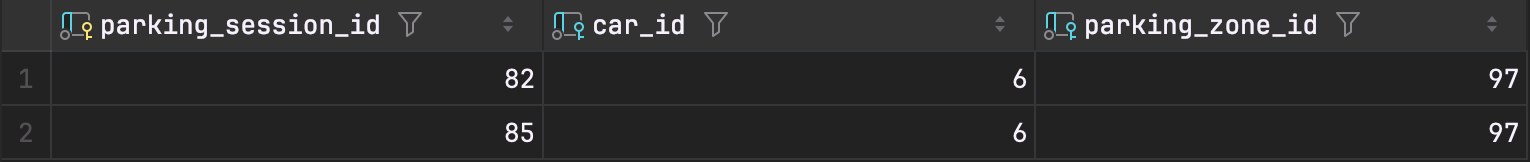
\includegraphics[width=0.5\linewidth]{myPhoto/trigger-9.png}
    \caption{Результат запроса: идентификаторы парковочных сессий выбранного автомобиля в выбранной зоне}
    \label{fig:trigger-9}
\end{figure}

Сначала удаляются все сессии выбранной зоны, кроме одной: счётчик не должен
измениться. После удаления последней сессии значение \textbf{parking\_count}
должно уменьшиться на единицу.

\begin{lstlisting}[style=sqlstyle, caption={Исходная статистика парковок}, label={lst:check-parking-before}]
SELECT car_id, parking_count
FROM car_stats
WHERE car_id = 6;
\end{lstlisting}

\begin{figure}[H]
    \centering
    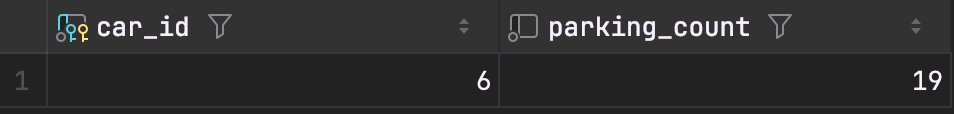
\includegraphics[width=0.5\linewidth]{myPhoto/trigger-10.png}
    \caption{Исходная статистика парковок}
    \label{fig:trigger-10}
\end{figure}

\begin{lstlisting}[style=sqlstyle, caption={Удаление всех сессий зоны, кроме одной}, label={lst:check-parking-delete-not-last}]
DELETE FROM parking_session
WHERE car_id = 6
  AND parking_zone_id = 97
  AND parking_session_id <> 82;
\end{lstlisting}

\begin{lstlisting}[style=sqlstyle, caption={Проверка после удаления не последней сессии}, label={lst:check-parking-after-not-last}]
SELECT car_id, parking_count
FROM car_stats
WHERE car_id = 6;
\end{lstlisting}

\begin{figure}[H]
    \centering
    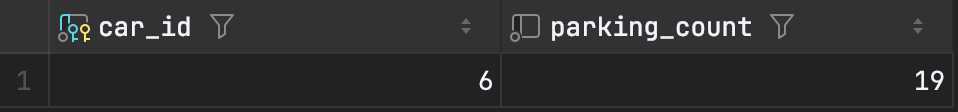
\includegraphics[width=0.5\linewidth]{myPhoto/trigger-11.png}
    \caption{Результат запроса: \texttt{parking\_count} не изменился после удаления всех сессий зоны, кроме одной}
    \label{fig:trigger-11}
\end{figure}

\begin{lstlisting}[style=sqlstyle, caption={Удаление последней сессии в зоне}, label={lst:check-parking-delete-last}]
DELETE FROM parking_session
WHERE parking_session_id = 82;
\end{lstlisting}

\begin{lstlisting}[style=sqlstyle, caption={Проверка после удаления последней сессии}, label={lst:check-parking-after-last}]
SELECT car_id, parking_count
FROM car_stats
WHERE car_id = 6;
\end{lstlisting}

\begin{figure}[H]
    \centering
    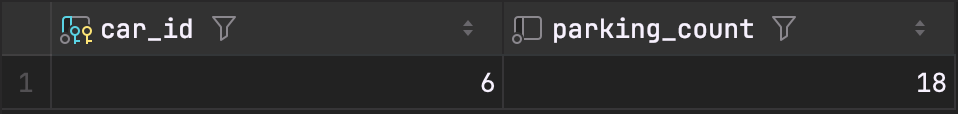
\includegraphics[width=0.5\linewidth]{myPhoto/trigger-12.png}
    \caption{Результат запроса: \texttt{parking\_count} уменьшился на 1 после удаления последней сессии}
    \label{fig:trigger-12}
\end{figure}

\subsubsection*{Проверка каскадного удаления парковочной зоны}
Отдельный триггер на таблицу \textbf{parking\_zone} не создаётся. Внешний
ключ в таблице \textbf{parking\_session} имеет правило
\textbf{ON DELETE CASCADE}, поэтому при удалении зоны PostgreSQL удаляет её
парковочные сессии. Для каждой удаляемой сессии запускается триггер
\textbf{parking\_session\_before\_delete}, который обновляет
\textbf{parking\_count}.

Для проверки выбирается зона, в которой имеется хотя бы одна парковочная
сессия. Необходимо сохранить значения \texttt{car\_id} и
\texttt{parking\_zone\_id}.

\begin{lstlisting}[style=sqlstyle, caption={Поиск данных для проверки каскадного удаления}, label={lst:find-zone-for-cascade}]
SELECT
    car_id,
    parking_zone_id
FROM parking_session
GROUP BY car_id, parking_zone_id
LIMIT 1;
\end{lstlisting}

\begin{figure}[H]
    \centering
    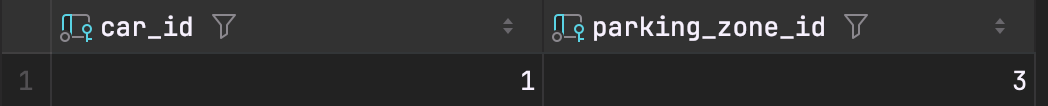
\includegraphics[width=0.5\linewidth]{myPhoto/trigger-13.png}
    \caption{Результат запроса: идентификаторы автомобиля и парковочной зоны для проверки каскадного удаления}
    \label{fig:trigger-13}
\end{figure}

Перед удалением зоны фиксируется исходная статистика выбранного автомобиля.

\begin{lstlisting}[style=sqlstyle, caption={Исходная статистика автомобиля}, label={lst:check-zone-before}]
SELECT car_id, parking_count
FROM car_stats
WHERE car_id = 1;
\end{lstlisting}

\begin{figure}[H]
    \centering
    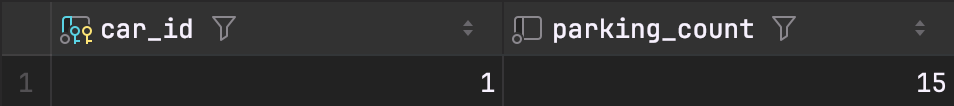
\includegraphics[width=0.5\linewidth]{myPhoto/trigger-14.png}
    \caption{Таблица \texttt{car\_stats} до удаления парковочной зоны}
    \label{fig:trigger-14}
\end{figure}

\begin{lstlisting}[style=sqlstyle, caption={Удаление парковочной зоны}, label={lst:delete-parking-zone}]
DELETE FROM parking_zone
WHERE parking_zone_id = 3;
\end{lstlisting}

После удаления зоны связанных с ней сессий в таблице
\textbf{parking\_session} быть не должно.

\begin{lstlisting}[style=sqlstyle, caption={Проверка каскадного удаления сессий}, label={lst:check-zone-sessions}]
SELECT *
FROM parking_session
WHERE parking_zone_id = 3;
\end{lstlisting}

\begin{figure}[H]
    \centering
    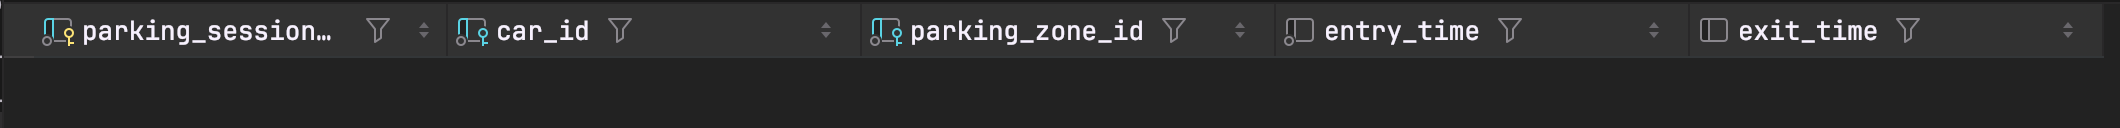
\includegraphics[width=0.5\linewidth]{myPhoto/trigger-15.png}
    \caption{Парковочные сессии удалённой зоны отсутствуют в таблице \texttt{parking\_session}}
    \label{fig:trigger-15}
\end{figure}

В результате значение \textbf{parking\_count} выбранного автомобиля должно
уменьшиться на единицу.

\begin{lstlisting}[style=sqlstyle, caption={Проверка статистики после удаления зоны}, label={lst:check-zone-after}]
SELECT car_id, parking_count
FROM car_stats
WHERE car_id = 1;
\end{lstlisting}

\begin{figure}[H]
    \centering
    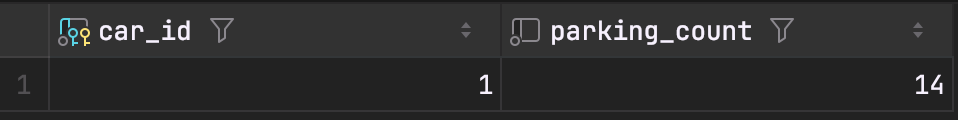
\includegraphics[width=0.5\linewidth]{myPhoto/trigger-16.png}
    \caption{Таблица \texttt{car\_stats} после удаления парковочной зоны: \texttt{parking\_count} уменьшился на 1}
    \label{fig:trigger-16}
\end{figure}

\newpage
